\section{Continuity}

The next idea we will develop is that of `continuity'. 

\subsection{Continuity of Functions}

Continuity is all about the behaviour of a function around a point. For a function to be be continuous at some $x$, we need $f(y)$ to be close to $f(x)$ whenever $y$ is sufficiently close to $x$.

\begin{definition}[Continuity]
	Let $A \subseteq \C$ and $f: A \rightarrow \C$. We say that $f$ is \vocab{continuous at $a$} $\in A$ if given any $\varepsilon > 0$ we can find a $\delta > 0$ s.t. $|f(x) - f(y)| < \varepsilon$ for all $y \in A$ s.t. $|x - y| < \delta$.


	We say that $f$ is \vocab{continuous} if it is continuous at every $a \in A$.
\end{definition}

You may notice that this definition uses exactly the definition of the limit of a function mentioned in \autoref{sec:lim-of-func}. This immediately gives us two more equivalent definitions of continuity.

\begin{proposition}[Limit Definition of Continuity]
	Let $f: A \rightarrow \C$. Then $f$ is continuous at $a \in A$ if and only if $\displaystyle \lim_{z \to a} f(z) = f(a)$.
\end{proposition}

\begin{proposition}[Sequence Definition of Continuity]
	Let $f : A \rightarrow \C$. Then $f$ is continuous at $a \in A$ if and only if for every sequence $a_n \in A$ with $a_n \rightarrow a$ we have $f(a_n) \rightarrow f(a)$.
\end{proposition}
% \begin{proof} \emph{Continuity Implies Sequential Continuity}.
% 	Given $\varepsilon > 0$, since $f$ is continuous at $a$, there exists $\delta > 0$ s.t. for all $x \in A$ with $|x - a| < \delta$ we have $|f(x) - f(a)| < \varepsilon$.
% 	So if $a_n \in A$ is a sequence with $a_n \rightarrow a$, there is an integer $N$ s.t. $n \geq N$ implies that $|a_n - a| < \delta$. Thus for $n \geq N$ we also have $|f(a_n) - f(a)| < \varepsilon$. So $f(a_n) \rightarrow f(a)$.

% 	\emph{Sequential Continuity Implies Continuity}.
% 	Suppose $f$ was not continuous at $a$. Then there exists an $\varepsilon > 0$ s.t. for all $\delta > 0$ there is some $y \in A$ with $|y - a| < \delta$ and $|f(y) - f(a)| \geq \varepsilon$.
% 	Then for each $\delta = 1/n$, we can find some $a_n$ s.t. $|a_n - a| < 1/n$ but $|f(a_n) - f(a)| \geq \varepsilon$. Then $a_n \rightarrow a$ but $f(a_n) \not\rightarrow f(a)$, which is a contradiction.
% \end{proof}

Each of the definitions have various advantages or disadvantages.
Still it is worth noting that the sequential/limit continuity definitions can be used to quite easily show certain properties of continuity that would otherwise be quite fiddly with the $\varepsilon$-$\delta$ definition. Using sequential continuity is also a natural way to show that a function \emph{is not} continuous at a point.
Let's take a look at some examples.

\begin{example}[The Constant Function is Continuous]
	If $f(x) = c$ then $f$ is continuous. To see this, we can take any value of $\delta$ in the definition.
	\end{example}

\begin{example}[$f(x) = x$ is Continuous]
	If $f(x) = x$ then $f$ is continuous. To see this, we can take $\delta = \varepsilon$ in the definition.
	\end{example}

\begin{example}[Step Functions are Discontinuous]
	Consider the function $f : \R \rightarrow \R$ with
	$$
	f(x) = \begin{cases}
        -1 &\mbox{if } x < 1, \\
        1 &\mbox{if } x \geq 1.
       \end{cases}
	$$
	\begin{center}
		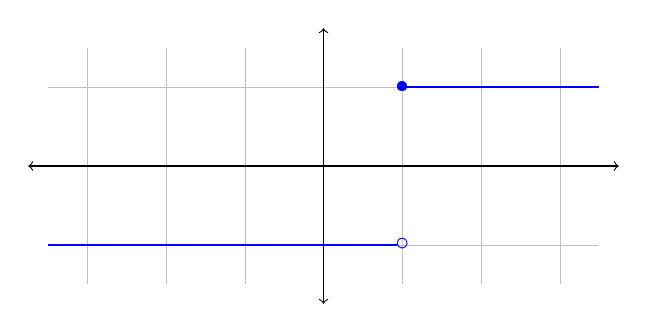
\begin{tikzpicture}
	  \draw[ultra thin,color=lightgray] (-3.5,-1.5) grid (3.5,1.5);   % coordinate grid
	  \draw[<->] (-3.75,0) -- (3.75,0);% node[right] {$x$};   % x-axis
	  \draw[<->] (0,-1.75) -- (0,1.75);% node[above] {$y$};   % y-axis
	
	%   \foreach \x/\xtext in {-4,...,-1,1,2,3,4}        % x-axis labels
	%   \draw (\x,2pt) -- (\x,-2pt) node[anchor=north, font=\footnotesize] {$\xtext$}; 
	
	%   \foreach \y/\ytext in {-4,..., -1,1,2,3, 4}           % y-axis labels
	%   \draw (2pt,\y) -- (-2pt,\y) node[anchor=east, font=\footnotesize] {$\ytext$}; 
	
	  % parametric function alpha(t)
	%   \draw [thick, samples=100,smooth] plot[variable=\t, domain=0:2*pi] ({3*cos(\t r)^3},{3*sin(\t r)^3});

	\draw [thick, samples=100,smooth, color=blue] plot[variable=\t, domain=-3.5:0.935] ({\t, -1});
	\draw [thick, samples=100,smooth, color=blue] plot[variable=\t, domain=1:3.5] ({\t, 1});

	\node at (1, -1) {\color{blue} $\circ$};
	\node at (1, 1) {\color{blue} \textbullet};
	
	\end{tikzpicture}
	\end{center}

	This function is not continuous at $1$. To see this, note that $1 - 1/n \rightarrow 1$ but $f(1 - 1/n) \rightarrow -1 \neq f(1)$ as $n \rightarrow \infty$.
\end{example}

\begin{example}[The Domain Matters]
Consider the function $f: \Q \rightarrow \R$ with
$$
\begin{cases}
	1 &\mbox{if } x^2 > 2, \\
	0 &\mbox{if } x^2 < 2.
   \end{cases}
$$
This function is continuous, since for every $a \in \Q$ there is an interval about $a$ for which $f$ is constant, so $f$ is continuous at $a$. If $f$ was defined on $\R$ instead of $\Q$, then it would be discontinuous only at $\pm\sqrt{2}$. But these points are not in our domain, so we don't need to worry about them.
\end{example}


\begin{example}[Continuity of $\sin 1/x$]\label{ex:sin-cont}
	Consider the function\footnote{I know that we haven't defined what $\sin$ is, but we will use it in examples because they are instructive. If this bothers you, feel free to come back after our discussion of power series.} $f: \R \rightarrow \R$ with $f(x) = \sin(1/x)$ if $x \neq 0$ and $f(0) = 0$.

	\begin{center}
		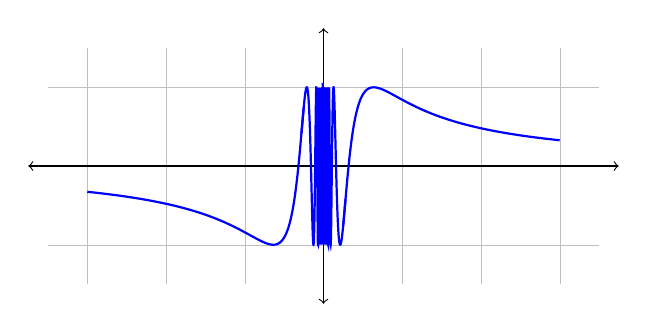
\begin{tikzpicture}
	  \draw[ultra thin,color=lightgray] (-3.5,-1.5) grid (3.5,1.5);   % coordinate grid
	  \draw[<->] (-3.75,0) -- (3.75,0);% node[right] {$x$};   % x-axis
	  \draw[<->] (0,-1.75) -- (0,1.75);% node[above] {$y$};   % y-axis
	
	%   \foreach \x/\xtext in {-4,...,-1,1,2,3,4}        % x-axis labels
	%   \draw (\x,2pt) -- (\x,-2pt) node[anchor=north, font=\footnotesize] {$\xtext$}; 
	
	%   \foreach \y/\ytext in {-4,..., -1,1,2,3, 4}           % y-axis labels
	%   \draw (2pt,\y) -- (-2pt,\y) node[anchor=east, font=\footnotesize] {$\ytext$}; 
	
	  % parametric function alpha(t)
	%   \draw [thick, samples=100,smooth] plot[variable=\t, domain=-3:3] (\t,sin(1/t));

	% \draw [thick, samples=100,smooth, color=blue] plot[variable=\t, domain=-3.5:0.935] ({\t, -1});
	% \draw [thick, samples=100,smooth, color=blue] plot[variable=\t, domain=1:3.5] ({\t, 1});

	\draw [thick, samples=100,smooth, color=blue] plot[variable=\t, domain=-3:-0.25] ({\t},{sin((\t)^(-1) r)});
	\draw [thick, samples=300,smooth, color=blue] plot[variable=\t, domain=-0.28:-0.005] ({\t},{sin((\t)^(-1) r)});
	\draw [thick, samples=300,smooth, color=blue] plot[variable=\t, domain=0.005:0.28] ({\t},{sin((\t)^(-1) r)});
	\draw [thick, samples=100,smooth, color=blue] plot[variable=\t, domain=0.25:3] ({\t},{sin((\t)^(-1) r)});
	% \draw [thick, samples=100,smooth] plot[variable=\t, domain=0.0001:3] (\t,{sin(1/t)});
	% \node at (1, -1) {\color{blue} $\circ$};
	% \node at (1, 1) {\color{blue} \textbullet};
	
	\end{tikzpicture}
	\end{center}
	This function is not continuous at $x = 0$. To see this, consider the sequence $a_n = \frac{1}{2\pi n + \pi/2}$. Then $a_n \rightarrow 0$, but $f(a_n) = 1 \rightarrow 1 \neq f(0)$ as $n \rightarrow \infty$.
\end{example}

\begin{example}[A Functional Equation with Continuity]
	We wish to find all continuous functions $f: \R \rightarrow \R$  s.t. $f(x) + f(2x) = 0$.

	Letting $x = 0$ we get $f(0) = 0$. Then rearranging we have
	$f(x) = -f(x/2)$, and repeatedly using this gives
	$$
	f(x) = -f\left(\frac{x}{2}\right) = f\left(\frac{x}{4}\right) = -f\left(\frac{x}{8}\right) = \cdots = (-1)^{n}f\left(\frac{x}{2^n}\right).
	$$
	Then since $f$ is continuous we have $f(x) = \lim_{n \to \infty} (-1)^n f(x/2^n) = f(0) = 0$. Thus $f(x) = 0$ is the only such function, which clearly works.
\end{example}


When attempting to determine if a function is continuous, one should keep in mind the following properties of continuity (all of which follow directly from our basic properties of limits).

\begin{proposition}[Sums, Products and Reciporicals of Continuous Functions]
	Let $f, g: A \rightarrow \C$ be functions. Then the following hold.
	\begin{enumerate}[label=(\roman*)]
		\item If $f$ and $g$ are continuous at $a$, then so is their sum $f + g$.
		\item If $f$ and $g$ are continuous at $a$, then so is their product $fg$.
		\item If $f$ is continuous at $a$ and $f(a) \neq 0$ then so is $1/f$.
	\end{enumerate}
\end{proposition}
\begin{proof}
	We prove each individually using the limit definition of continuity.
	\begin{enumerate}[label=(\roman*)]
		\item If $\displaystyle\lim_{z \to a} f(z) = f(a)$ and $\displaystyle\lim_{z \to a} g(z) = g(a)$ then $\displaystyle\lim_{z \to a} (f+g)(z) = (f+g)(a)$.
		\item If $\displaystyle\lim_{z \to a} f(z) = f(a)$ and $\displaystyle\lim_{z \to a} g(z) = g(a)$ then $\displaystyle\lim_{z \to a} (fg)(z) = (fg)(a)$.
		\item If $\displaystyle\lim_{z \to a} f(z) = f(a)$ and $f(a) \neq 0$, then $\displaystyle\lim_{z \to a} 1/f(z) = 1/f(a)$.
		 \qedhere
	\end{enumerate}
	% \begin{enumerate}[label=(\roman*)]
	% 	\item If $a_n \in A$ and $a_n \rightarrow a$, then $(f + g)(a_n) = f(a_n) + g(a_n) \rightarrow f(a) + g(a) = (f + g)(a)$ as $n \rightarrow \infty$. So $f + g$ is continuous at $a$.
	% 	\item If $a_n \in A$ and $a_n \rightarrow a$, then $(fg)(a_n) = f(a_n)g(a_n) \rightarrow f(a)g(a) = (fg)(a)$ as $n \rightarrow \infty$. So $fg$ is continuous at $a$.
	% 	\item If $a_n \rightarrow a$ and $f(a_n) \neq 0$ for all $n$, then $1/f(a_n) \rightarrow 1/f(a)$. So $1/f$ is continuous at $a$. \qedhere
	% \end{enumerate}
\end{proof}

Along with the fact that $f(x) = x$ and $f(x) = c$ are continuous, these properties imply that all polynomials are continuous.


\begin{proposition}[The Composition of Continuous Functions is Continuous]
	Let $f: A \rightarrow B$ and $g: B \rightarrow \C$ with $A, B \subseteq \C$. Then if $f$ is continuous at $a \in A$ and $g$ is continuous at $f(a)$, then $g \circ f$ is also continuous at $a$.
\end{proposition}
\begin{proof}
	If $a_n \rightarrow a$ then by the continuity of $f$ we have $f(a_n) \rightarrow f(a)$, and by the continuity of $g$ we have $g(f(a_n)) \rightarrow g(f(a))$. So $g\circ f$ is continuous at $a$.
\end{proof}

\subsection{The Intermediate Value Theorem}

Continuous functions are nice because they have a few nice properties. The first of these that we will prove is the \emph{intermediate value theorem}, a central theorem in elementary analysis. The idea of the intermediate value theorem is that if a continuous function starts at one value and ends at a different value, then it must take on all of the values in between.

\begin{center}
	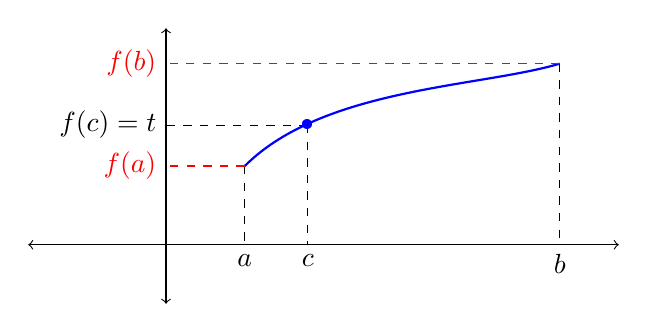
\begin{tikzpicture}
%   \draw[ultra thin,color=lightgray] (-3.5,-0.5) grid (3.5,2.5);   % coordinate grid
  \draw[<->] (-3.75,0) -- (3.75,0);% node[right] {$x$};   % x-axis
  \draw[<->] (-2,-0.75) -- (-2,2.75);% node[above] {$y$};   % y-axis

%   \foreach \x/\xtext in {-4,...,-1,1,2,3,4}        % x-axis labels
%   \draw (\x,2pt) -- (\x,-2pt) node[anchor=north, font=\footnotesize] {$\xtext$}; 

%   \foreach \y/\ytext in {-4,..., -1,1,2,3, 4}           % y-axis labels
%   \draw (2pt,\y) -- (-2pt,\y) node[anchor=east, font=\footnotesize] {$\ytext$}; 

  % parametric function alpha(t)
%   \draw [thick, samples=100,smooth] plot[variable=\t, domain=0:2*pi] ({3*cos(\t r)^3},{3*sin(\t r)^3});

% \draw [thick, samples=100,smooth, color=blue] plot[variable=\t, domain=-3.5:0.935] ({\t, -1});
% \draw [thick, samples=100,smooth, color=blue] plot[variable=\t, domain=1:3.5] ({\t, 1});

% \node at (0, 0) {\color{blue} $\textbullet$};


%Curve Lines [id:da5569099817019642] 
\draw[thick, smooth, color=blue]    (-1,1) .. controls (0,2) and (2,2) .. (3,2.3) ;

\draw  [dashed] (-1, 1) -- (-1, 0) node [below] {$a$};
% \node at (-1, 0) {$a$};
\draw  [dashed, ] (3, 2.3) -- (3, 0) node [below] {$b$};

\draw  [dashed, red] (3, 2.3) -- (-2, 2.3) node [left] {$f(b)$};
\draw  [dashed, red] (-1, 1) -- (-2, 1) node [left] {$f(a)$};
% \node at (3, 0) {$b$};

\draw  [dashed] (-0.2, 1.52) -- (-0.2, 0) node [below] {$c$};
\draw  [dashed] (-0.2, 1.52) -- (-2, 1.52) node [left] {$f(c)=t$};

\node at (-0.2, 1.52) {\color{blue}\small \textbullet};





\end{tikzpicture}
\end{center}

In the proof below we will employ suprema\footnote{If you are unfamiliar with this term and/or the least upper bound principle, feel free to have a look at Chapter 2 of my `Numbers and Sets' course notes.}, but we will give another proof afterwards that does not use this (at the expense of being slightly longer).

\begin{theorem}[The Intermediate Value Theorem]
	Let $f: [a, b] \rightarrow \R$ be a continuous function. Then for every $t$ between $f(a)$ and $f(b)$ there is an $c \in [a, b]$ with $f(c) = t$.
\end{theorem}
\begin{proof}
Suppose without loss of generality\footnote{If $t = f(a)$ or $t = f(b)$ then we are done. Also the case $f(a)> t> f(b)$ follows similarity.} that $f(a) < t < f(b)$. Consider the set $S = \{x \in [a, b] : f(x) < t\}$. This set is bounded and since $a \in S$ it is non-empty. So we can let $c = \sup S$, and note that $a \leq c \leq b$.

Let $n \geq 1$ be an integer. Then since $c$ is the supremum there must exist some $x_n \in S$ s.t. $c - \frac{1}{n} < x_n \leq c$. 
By the squeeze theorem we have $x_n \rightarrow c$ as $n \rightarrow \infty$.
Also $f$ is continuous so $f(x_n) \rightarrow f(c)$. 
We also constructed $x_n$ to be in $S$, giving $f(x_n) < t$ for all $n$. This implies that $f(c) \leq t$. 

We know that $c \in [a, b]$ but $c \neq b$, so there is some integer $N$ s.t. for $n \geq N$ we have $c + 1/n \leq b$.
Using that $c$ is the supremum, we have $c + 1/n \not \in S$ for all $n \geq N$, that is, $f(c + 1/n) \geq t$ for all $n\geq N$.
Then by continuity we have $f(c) \geq t$. 

But then $f(c) \geq t$ and $f(c) \leq t$, so we must have $f(c) = t$.
\end{proof}

Before we look at some examples of using the intermediate value theorem, there's a few things worth noting about the intermediate value theorem.

First of all, we say absolutely nothing about uniqueness in the theorem. It is very much possible for a function to take on an intermediate value multiple times.
Second of all, when applying the intermediate value theorem (commonly abbreviated to IVT) a good general problem solving technique is trying to apply IVT to other related functions such as $g(x) = f(x) - x$ or $g(x) = f(x) - t$ and things like that. You will see this `trick' show up in the examples below, and also again when we get to Rolle's theorem and the mean value theorem.


\begin{example}[Fixed Points of Continuous Maps from ${[0,1]}$ to Itself]
	We will prove that if $f:[0, 1] \rightarrow [0, 1]$ is a continuous function then there is some $c \in [0, 1]$ s.t. $f(c)=c$.

	Consider the function $g(x) = f(x) - x$. Then $g$ is continuous with $g(0) = f(0)$ and $g(1) = f(1) - 1$. 
	Since $0 \leq f(x) \leq 1$, we must have $g(0) \geq 0$ and $g(1) \leq 0$. Thus by the intermediate value theorem there exists some $c \in [0, 1]$ s.t. $g(c) = 0$. But then we have $f(c) - c = 0$, that is, $f(c) = c$ as required.
\end{example}

\begin{example}[Existence $n$th Roots]
	We will show that for any positive integer $n$ and $y > 0$ there exists a real number $x$ s.t. $x^n = y$.

	Consider the function $f(x) = x^n$. This function is continuous on $[0, 1 + y]$, and since $f(0) = 0$ and $f(1 + y) = (1 + y)^n$, we have $f(0) < y < f(1 + y)$.
	Thus by the intermediate value theorem there is some $x \in [0, 1+ y]$ s.t. $f(x) = y$, that is, $x^N = y$.
\end{example}

Now before we look on let's have a look at an alternative proof for the intermediate value theorem. This proof uses the same idea as the previous proof (try to see why) but avoids the use of suprema.

\begin{aside}{Aside: Hunting For \st{Lions} Intermediate Values}
	It was mentioned before that the `lion hunting' technique that we used to prove the Bolzano–Weierstrass theorem could also be used to prove other theorems in Analysis. One such example is the intermediate value theorem.

	The steps in the proof are quite similar to that of the proof of the Bolzano-Weierstrass theorem, the only difference is what we are `hunting for', which in this case is our intermediate value, and how we finish off the proof.

	\begin{proof}[Proof (Intermediate Value Theorem, Lion Hunting Style)]
Again suppose without loss of generality that $f(a) < t < f(b)$.
We are going to define two sequences $a_n$ and $b_n$ inductively as follows. Begin by setting $a_1 = a$ and $b_1=b$, and let $c = (a_1 + b_1)/2$ be the midpoint $a_1$ and $b_1$.

Then there is two possibilities:
\begin{enumerate}
\item $f(c_1) \geq t$.
\item $f(c_1) < t$.
\end{enumerate}
If the first one holds, we set $a_2 = a_1$ and $b_2 = c_1$, and if it doesn't then we set $a_2 = c_1$ and $b_2 = b_1$.
Repeating this process, we construct $a_n$ and $b_n$ s.t. $f(a_n) \leq t \leq f(b_n)$, $a_{n - 1} \leq a_n \leq b_n \leq b_{n - 1}$, and also $b_n - a_n = (b_{n - 1} - a_{n - 1})/2$.

Now $a_n$ is increasing and bounded above, and $b_n$ is decreasing and bounded below and thus $a_n \rightarrow c \in [a, b]$, and $b_n \rightarrow c' \in [a, b]$. Then we have $c - c' = (c - c')/2$ using the above result, and thus $c = c'$.

Since $f$ is continuous at $c$ and $a_n \rightarrow c$, we know that $f(a_n) \rightarrow c$ as $n \rightarrow \infty$. Since $f(a_n) \leq t$, we also know that $f(c) \leq t$. Similarity we also have $f(b_n) \geq t$, so $f(c) \geq t$. But then $t \leq f(c) \leq t$, and thus $f(c) = t$, and we are done.
	\end{proof}

	To get a feel for the construction, try drawing a rough sketch of the process. If you consider the case of a function that takes on the desired intermediate value multiple times, you should also see the that this proof does not give the same value for $c$ as the previous proof.

\end{aside}


A natural question upon learning of the intermediate value theorem is if it is equivalent to definition of continuity. The answer to this question is no -- there are functions that have the `intermediate value property', without being continuous. One example is $\sin(1/x)$ which we showed is discontinuous at $x = 0$ in \autoref{ex:sin-cont}. Another more elaborate example is `Conway's Base-13 Function', which has the intermediate value property but is discontinuous everywhere. You can read more about this function on \href{https://en.wikipedia.org/wiki/Conway_base_13_function}{Wikipedia}.


\subsection{The Boundedness Theorem}

The last result about continuous functions that we will prove is the \emph{boundedness theorem}, another central theorem in elementary analysis. The statement of this result is straightforward: a continuous function on a closed bounded interval is bounded and attains its bounds.

First we will prove that a continuous function defined on some closed interval is indeed bounded.
\begin{lemma}[Continuous Function on Closed Interval is Bounded]
	If $f:[a, b] \rightarrow \R$ is continuous then there exists $K$ s.t. $|f(x)| \leq K$ for all $x \in [a, b]$.
\end{lemma}
\begin{proof}
If $f$ was unbounded, then given any integer $n \geq 1$ there exists $x_n \in [a, b]$ s.t. $|f(x_n)| > n$. By Bolzano–Weierstrass, $x_n$ has a convergent subsequence $x_{n_j} \rightarrow x$. Also since $a \leq x \leq b$, we must have $x \in [a, b]$.
By continuity of $f$, $f(x_{n_j}) \rightarrow f(x)$, but $|f(x_{n_j})| > n_j$, and thus does not tend to a limit. Thus we have a contradiction.
\end{proof}

Now we can prove that such a continuous function attains its bounds, giving us the boundedness theorem.

\begin{theorem}[Boundedness Theorem]
	If $f:[a, b] \rightarrow \R$ is continuous then there exists $x_1, x_2 \in [a, b]$ s.t. $f(x_1) \leq f(x) \leq f(x_2)$ for all $x \in [a, b]$.
\end{theorem}
\begin{proof}
	By our previous lemma, we know that $f$ is bounded. Now we define the set
	$$
	A = \{f(x) : x \in [a, b]\}.
	$$
	This set is bounded and non-empty and thus has a supremum $M = \sup A$. Then for each positive integer $n$, $M - 1/n$ cannot be an upper bound for $A$. This implies that there is some $x_n \in [a, b]$ s.t. $M - 1/n < f(x_n) \leq M$.

	By Bolzano–Weierstrass, $x_n$ has a convergent subsequence $x_{n_j} \rightarrow x$. Since $a \leq x_n \leq b$, we know $a \leq x \leq b$. By the continuity of $f$, $f(x_{n_j}) \rightarrow f(x)$, but $f(x_{n_j}) \rightarrow M$ by construction. 
	So $f(x) = M$. So $x_2 = x$. The minimum follows analogously. \qedhere

	\emph{Alternate Proof}. As before, let $M = \sup A$ and suppose that there was no $x_2$ s.t. $f(x_2) = M$. Then let $g(x) = \frac{1}{M - f(x)}$ for $x \in [a, b]$. This function is well defined and continuous. Now $g$ must be bounded by the previous lemma, so $g(x) \leq K$ for all $x \in [a, b]$, for some $K$. This means that $f(x) \leq M - 1/k$ on $[a, b]$. This is contradiction since we set $M$ as the supremum. \hfill\qed
\end{proof}

\clearpage